\documentclass[12pt]{article}

\usepackage{graphicx}

\title{\textbf{TetrAIs}\\ {\small Search Based Artificial Intelligence Program for Autonomous Tetris Gameplay}}
\author{Saagar Deshpande, Louis Li, Brandon Sim\\ {\small Computer Science 182, Harvard University}}
\usepackage{hyperref}

\begin{document}
\maketitle
\tableofcontents
\newpage

\section{Introduction}
TetrAIs is an artificial intelligence agent which plays the well-known game of Tetris. The game is played on a 20 $\times$ 10 board of empty cells, which is filled by tetrominoes, geometric shapes connected by four squares connected orthogonally. The offline version of the game, in which the order of subsequent pieces is known, has been proven to be NP complete via reduction to the 3-partition problem [5]. In addition, the online version, in which subsequent pieces are randomly chosen, is also difficult, because the piece that the computer ``plays'' is unknown.

Tetris is a complex game with an extremely large search space, making even the simplest of AIs slow to compete on the standard game board. A standard Tetris board contains $10\times 20 = 200$ cells, each of which can be either filled or empty, placing a maximum bound of $2^{200}$ on the total number of possible board configurations. Further, we note that each added tetromino adds 4 filled spaces to the board, and each line removed will remove 10 filled spaces from the board. 

Using these basic constraints, we note that the number of filled spaces on the board will always be even, removing half of the possible configurations, providing a new upper bound of $2^{199}$ or approx $8\cdot 10^{59}$ configurations for the board. In our paper, we show that using a combination of heuristics, we are able to create an AI with strength comparable to that of the best human players, clearing over 2500 lines. We note that there is some room for improving the AI, as our implementation does not take into consideration any potential piece swaps and the ability to slide pieces after soft dropping, which limits the search space, providing a more reasonable project for our timeline.

\subsection{Definitions and Terminology}
Below are some definitions and terms which will be used throughout the paper:
\begin{enumerate}
\item \textbf{Empty Square} - A square on the game board which is not filled by a part of a tetromino.
\item \textbf{Full Square} - A square on the game board which is filled by a part of a tetromino.
\item \textbf{Fringe} - The set of spaces where the next piece may be placed.
\item \textbf{Game Stack} - The set of all frozen pieces on the board at any given time. Pieces are considered frozen as soon as a falling piece touches either the bottom of the game board or another piece on the game stack.
\item \textbf{Cleared Line} - A line which has all 10 blocks filled in horizontally. This line will be ``cleared'' or removed from the game board. All blocks above this line will fall one square down, reducing the height of the puzzle, and the player is given points for this action.
\item \textbf{Tetris} - 4 simultaneously cleared lines. A tetris occurs when 4 lines are cleared at the same time. The player gets points for this action, more than clearing 4 lines with more than 1 piece.
\item \textbf{Piece} - A tetronimo. These are pieces which are used in the game. Playing a piece gives the player some number of points. Typically, this is the lowest number of points you can score in the game.
\item \textbf{Soft Drop} - A piece that is allowed to reach the fringe using the game gravity. In standard play, this piece may slide around the fringe for a few seconds provided there are no height constraints blocking movement. This is not implemented for our AI.
\item \textbf{Hard Drop} - A piece that is dropped instantly from its location to the fringe. Hard dropped pieces freeze where they land.
\end{enumerate}


\section{Background and Motivation}
\subsection{Motivation}
The motivation behind our paper was to create an AI that would be able to play a simple version of Tetris and play it better than the average human player. In numerous anecdotal trials, the authors of this paper scored with varying results, maxing out at around 100 lines. Because Tetris has such a high computational complexity, this paper aimed to create an AI that would be able to place pieces within a reasonable timespan, allowing for it to be theoretically competitive with human players in a standard game environment. 

\subsection{Goals}
For our AI, we decided that we would focus on maximizing the number of lines cleared, with preference given to clearing Tetrises, or 4 lines simultaneously. This is because most research literature compares the number of lines cleared, using that as a metric for success. The goals are as follows:
\begin{enumerate}
\item Maximize the number of lines cleared before losing the game.
\item Provide ability to lookahead. That is, if our lookahead is set to 1, we are playing by looking at the current piece. We want our AI to be able to compute the best move by looking ahead at least 1 piece (lookahead = 2). This is comparable to [7]. We also want to be able to lookahead further if computationally feasible, or at least provide the framework to do so.
\item Provide game replayability. We want to be able to save and replay (watch) games generated by the AI. This will allow us to visually evaluate the success of our heuristics and also construct weighted evaluation.
\end{enumerate}

\subsection{Scope}
Because live Tetris is an NP-complete problem [1], we decided to play offline Tetris, which is a game variant in which all pieces are known at the game’s start. However, more research found that this variant is NP-complete as well [5], with metrics that are merely approximations at best. Using these papers as a starting point, we decided to limit the scope of our AI to the following constraints:
\begin{enumerate}
\item No soft drop and fringe sliding - We decided that we would limit the search space of the problem by only allowing hard drops of pieces onto the board. This means that once a piece is played, it is frozen and can’t be moved. This constraint is important because pathfinding on the Tetris game board is a fairly computational problem to solve.
\item No piece save and swap - A typically feature found in Tetris is the ability to save a piece for later use. A player can swap between the current piece and the saved piece once per new piece, allowing for greater line clearing ability. We did not include this feature for computational reasons; with an AI lookahead of 2, which is similar to a swap situation, the game takes hours to complete.
\item Store up to 50 known pieces - Although we are playing offline Tetris, there is currently no way for us to use 50 pieces in a search tree, so we store up to 50 pieces for our game situation, and generate new pieces when we play old ones.
\item Focus on line clears and ignore score - Although scoring is a useful metric, most research literature measure performance via the number of lines cleared. The two metrics are clearly highly correlated.
\end{enumerate}

\subsection{Initial Algorithm Design and Computational Concerns}
We initially considered multiple algorithms for solving the AI Tetris problem, including A* search, reinforcement learning, and case-based reasoning [2][3]. However, after much discussions and experimentation with Python, we settled on a Greedy Local Search algorithm that would score each potential game state using various board-based heuristics [4][5][6]. Furthermore, we discovered that more complex heuristics provided better game play by the AI [7]. Thoughts on the feasibility and usefulness of lookahead were confirmed by additional research [7]. 

Initially, we were worried about the following factors in relation to computational feasibility of our Tetris AI.
\begin{enumerate}
\item Memory Limit: Because of the number of possible positions to place a piece, rotate a piece, and score a piece, we might not have enough memory to represent a game tree fully past a few levels.
\item Game Time Limit: Because the search space is quite large, as mentioned in the memory limit, we might not be fast enough to make a decision, especially as the game moves on. In Tetris, there is a time limit per piece, as the piece will automatically fall to make the game progress.
\item Tree Depth: In a true online game, we will not have a very deep tree search space because we will only know with 100\% accuracy the current piece and the next playable piece. This limits the depth of the tree; we will develop a expected value heuristic if necessary to counter this.
\end{enumerate}


\section{Algorithms and Data Structures}
\subsection{Algorithm}
\textbf{LOUIS}

\subsection{Data Structures}
For our implementation, we used Python and integrated our Tetrais code into an already existing Tetris game implementation. You can find the corresponding source mentioned in our codebase, however, most of the existing Tetris code was ripped out and replaced by Tetrais logic. 

We use a 2-D array, represented as a list of lists in Python, to represent the game board. We have generic block object to represent the shape of the block; this logic can be found in tetris.py and was borrowed from the existing implementation. A state is represented by a dict with keys "board" and "pieces", where "pieces" is the remaining pieces (thus piece[0] is the next piece).

\subsection{Heuristics}

For Tetrais, we implemented various heuristics to improve the AI’s ability to clear lines in the game. For our research, we break these heuristics down into two types: board properties and gameplay properties. Board properties are conditions that exist for every piece; that is, no matter which piece is played, the board will heuristically have the game state for every piece. Gameplay properties are more piece dependent, and are geared towards more specific scenarios.

\textbf{Board Properties}
\begin{enumerate}
\item Maximum height - This heuristic computes the maximum height of the board at any given time. More specifically, across all columns in the board, this value reflects that of the highest column.
\item Average height - This heuristic computes the average height across all columns of the board. Computationally, this is the sum of all heights across the columns, divided by the number of columns.
\item Underhangs or ``holes'' - This heuristic finds all empty spaces that have a filled square on top of it. More formally, a square $(x,y)$ is a hole if $(x,y)$ contains no piece and $(x, y+1)$ is filled with some piece.
\end{enumerate}

\textbf{Gameplay Properties}
\begin{enumerate}
\item Bumpiness - This heuristic measures the sum of the absolute height differences between neighboring columns. This heuristic is important because bumpiness can help some pieces and hurt others. For example, Z and S pieces are typically helped by bumpiness; the long I piece is not. However, ultimately, the initial game board is not bumpy at all, and it is most preferable to reach that game state if possible.
\item Valleys - This heuristic measures the number of spaces where only a line piece can fit. More formally, this is an empty space $(x, y)$ such that $(x, y+1)$ and $(x, y+2)$ are also empty, and $height(x-1) \geq y+3$ and $height(x+1) \geq y+3$ (neighboring columns are at least $y+3$ in height). Note that this heuristic can be relaxed for the L and J pieces by reducing the minimum height to $y+2$, and can be further relaxed for other pieces as well.
\end{enumerate}

The goal of the heuristic function is to minimize the heights, underhangs, bumpiness, and valleys, as we want to get as close to the initial state as possible while still clearing lines.

We initially used a simple heuristic that combined the board properties and placed an emphasis on the underhangs. This was demoed during the class presentation, and performed reasonably well; however, even minorly serious attempts by the authors were able to match the performance of this simple heuristic. Further research found Gameplay Properties [6,7]. This linear combination of the different evaluation metrics improved the Tetrais performance to over 2000 lines.

\textbf{Heuristic Evaluation Examples}

\begin{figure}[h!]
    \centering
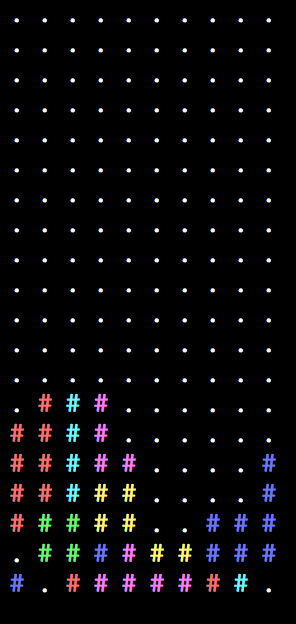
\includegraphics[height=2.0in]{bumpiness.png}
\caption{Example of a Tetris board}
\end{figure}

In the example Tetris board, we see how some of the heuristics work:
\begin{itemize}
    \item Maximum height - 7 (from the second, third, and fourth columns)
    \item Average height - The board has heights of $[6, 7, 7, 7, 5, 2, 2, 3, 3, 5]$. The average height is $47 / 10 = 4.7$. 
    \item Holes - 3
    \item Bumpiness -  The differences in heights are $[-1, 0, 0, 2, 3, 0, -1, 0, -2]$. We sum the absolute height differences to yield $1 + 2 + 3 + 1 + 2 = 9$.
    \item Valleys - There are no valleys on this board example board, since there is no space such that only a line piece can fit.
\end{itemize}

\section{Analysis}
\subsection{Results}
Below is a table of some of our results:\vspace{2em}

\begin{tabular}{|c|c|c|c|}\hline
Lookahead Depth & Heuristic & Average Lines Cleared & Trials\\ \hline
1 & Simple & 23.9 & 20\\ \hline
2 & Simple & 41.4 & 20\\ \hline
1 & Complex & 2361.5 & 2\\ \hline
2 & Complex & Code Still Running & -\\ \hline
\end{tabular}

\subsection{Evaluation}
Our initial attempts with the Tetrais algorithm resulted in fairly low scores. We provide results here to compare against later attempts. The simple heuristic in question was an un-optimized formula that took into consideration max height, average height, and number of holes/underhangs, with a higher penalty for the number of holes. These attempts were fueled by the following weak proof: In a Tetris game board, the fringe is always clearable. By clearing a line on the fringe, it is possible to reduce the size of the game stack, and lower the maximum height, thus allowing one to clear more lines. One property of a high scoring game is that the game stack is minimized whenever possible. However, if a hole or underhang appears, there is no possible move by which a piece played can reduce the game stack to 0, the smallest possible state. Thus, by allowing holes or underhangs to appear, the player moves further away from the safest and highest scoring game state. While this proof does not hold in all situations (one might research soft drop and piece sliding or the T-spin manuvuer - \url{http://tetris.wikia.com/wiki/T-Spin}) and is by no means rigorous, for our AI and game implementation, minimizing the number of holes allows us to maximize the playability of the board and thus the number of lines cleared by Tetrais.

The initial attempts with no lookahead (lookahead = 1) and simple heuristic resulted in average scores around 20 lines per game. This is around the level of gameplay of most novice players (as judged by relative gameplay at \url{http://www.tetrisfriends.com/leaderboard/index.php}). After running the simple heuristic with 1 piece lookahead, Tetrais was about to clear roughly 40 lines per game, with game highs of around 90 lines. This validates the results seen in [7] in that 1 piece lookahead provides better results, however, even minorly serious attempts by the authors were able to match the performance of this simple heuristic. 

We augmented the search algorithm and improved our heuristics, adding bumpiness and valleys as additional game metrics (Gameplay Heuristics [6,7]). Results from no lookahead with complex heuristics provides games scoring as high as 2600 lines. We find that this adequately plays the game of Tetris at an expert level. We note that the world record for humans is 4,988, with a variant of the game that includes piece swaps and the ability to slide pieces after soft drops [8]. As noted previously, these two features were left out of our implementation due to computational complexity. While they are not critical features in every standard implementation of Tetris, having the ability to swap pieces and slide pieces along the fringe would allow us greater range of moves and thus allow us to clear drastically more lines during game play. These two features alone would allow our algorithm to easily beat the human world record, as seen by the AI in [7], which scores 4000 times more in line clears alone, as even Tetris masters can not play with the precision and speed of an AI [7].

Finally, with a complex heuristic and 1 piece lookahead, we attempted to beat the previous algorithm. However, we ran 2 piece lookahead for many hours, as noted above, and the game has not yet finished. This could be due to slowness of code as well as its skill in playing, as it can be place many more pieces without dying (at which point the code will end).

\subsection{Critique and Concerns}
Although our algorithm has been tuned to provide better results with more complex heuristics, we have some outstanding critiques and concerns about Tetrais.
\begin{enumerate}
\item Time per move - Our python implementation (complex heuristic) takes longer to compute than expected. While games run around 10 minutes, many take much longer, even with 1 piece lookahead. On average, it takes roughly 1 second per piece played. We believe that our heuristic computations are somewhat expensive. Furthermore, we check every possible move; this might not be necessary for every step of the game.
\item Expense of Heuristic Computation - The heuristic computation iterates over the game board multiple times. This is not a very terrible cost because the game board is reasonably small, however, for Tetrais, this computation adds up very fast due to the number of pieces played. We might consider a better grid representation for the future, as well as faster techniques to evaluate the heuristics.
\item Inefficiency of lookahead - Lookahead adds an extra layer of computation that increases the Tetrais computation time by more than a factor of 4. It’s hard for us to measure the true impact, as most of our simulations did not finish running after 3-4 hours of continuous run time. However, verbose mode gives a reasonable indication as to the slow down, and we see hope that future experimentation will help us improve our lookahead approach. Finally, some additional testing is needed to ensure the correctness of our lookahead code.
\item Lack of case-based piece analysis - Regardless of tuning, there are some occasions where Tetrais will make a bad move for non-obvious reasons. A case-based piece analysis might yield better placement for some pieces in key situations. The heuristic prefers that long I pieces lay flat if there is no valley for it, however, most Tetris players prefer a vertical placement regardless. Case-based piece analysis would help with these situations, and may actually speed up gameplay if the heuristic is ignored for these situations.
\end{enumerate}

\section{Conclusion}
This paper presents an AI Tetris agent which uses a heuristically driven, greedy local search technique to optimize the number of lines cleared over the course of a game of Tetris. Our results show that with a complex heuristic and multiple heuristic factors, the Tetrais agent is able to compete against expert humans in the offline version of tetris, clearing more than 2600 lines at its best. While we were unable to really measure the true performance of the 2 piece lookahead version of Tetrais, we believe that this version will provide a significantly higher result. 

With additional time, here are some future directions that we would like to consider.
\begin{enumerate}
\item Soft drops and piece swaps - We want to enable piece drops and fringe sliding to improve the quality of our gameplay. By allowing for these two features, a variety of moves will be available to us that will enable more complex game play options and allow for us to clear more Tetrises.
\item Increase efficiency for lookahead by preprocessing - With additional experimentation, we believe that we might be able to derive a heuristic that will allow us to preprocess pieces. Some pieces and positions are just infeasible to look at, and a faster preprocessing function can help ignore these pieces.
\item Case-based piece analysis - Case-based analysis will allow us to place pieces correctly in situations where the heuristic returns a strong result which results in ambiguous play on the game board. The heuristic prefers that long I pieces lay flat if there is no valley for it, however, most Tetris players prefer a vertical placement regardless. Case-based piece analysis would help with these situations, and may actually speed up gameplay if the heuristic is ignored for these situations.
\end{enumerate}

\section{Appendix 1: Examples and Demonstrations}

\section{Appendix 2: Documentation}
\subsection{Prerequisites}
The only prerequisite is the \verb|colorama| library. It can be installed via \verb|pip| or \verb|easy_install| with the following:
\begin{verbatim}
pip install colorama
\end{verbatim}

\subsection{Usage}
In order to run the tetris solver, run:
\begin{verbatim}
python algo.py [OPTIONS]
   -h, --help      Prints this help dialog
   -t, --tetris    Runs the tetris AI simulation
        ARGS: [# trials] [lookahead = 1,2,...] [watch replay=0,1] [verbose=0,1]
   -r, --replay    Watch a game replay
        ARGS: [gamelog]
\end{verbatim}
At the end of each trial, you can print a replay of the game and the number of lines cleared if you enable watch replay. You can see a more verbose line clear if you enable verbose mode.

\begin{verbatim}
python algo.py -t 10 1 1 1
\end{verbatim}
This command will run the game with 10 trials, no lookahead, watching replays enabled after game ends, verbose output enabled.

\begin{verbatim}
python algo.py -r [gamelog]
\end{verbatim}
This command will replay a gamelog. Some sample gamelogs are available in the provided source files.

\section{Source Code}   
Source code can be found in the submitted \verb|.zip| file on the course dropbox and as well on Github at: \url{https://github.com/raysaagar/ai-tetris}

\section{References}
\begin{enumerate}
\item \url{http://citeseerx.ist.psu.edu/viewdoc/download?doi=10.1.1.102.8760&rep=rep1&type=pdf}
This paper describes the reduction of Tetris to the 3-PARTITION problem. This provides a useful way to frame a potential solver for the game.
\item \url{http://www.cs.ru.ac.za/research/g02C0108/files/litreviewfinalhandin.pdf}
This paper describes a strategy for solving using reinforcement learning (intuitively, trial-and-error learning). It also includes useful descriptions of potential vectors to describe the state space.
\item \url{http://www.ift.ulaval.ca/~lamontagne/pubs/flairs2008.pdf}
This paper also examines reinforcement, but it places an emphasis on case based reasoning. It evaluates the performance of an algorithm that employs case-based reasoning.
\item \url{https://www2.informatik.uni-erlangen.de/EN/publication/download/mic.pdf}
This paper examines a way to rate possible Tetris configurations (i.e. through a heuristic function) by dividing into 10 “subratings”, each corresponding to a feature of a Tetris configuration. The heuristic is the weighted sum of the subratings, and they provide an algorithm for determining the weights in the heuristic.
\item   \url{http://arxiv.org/pdf/cs.cc/0210020.pdf}
This paper proves that the “offline” version of Tetris, where the order of the pieces is known, is NP-complete. They further describe how a number of metrics can be used to devise a strategy, but even these are hard to approximate.
\item \url{http://www.cs.huji.ac.il/~lirchi/AIP/Tetris1.pdf}
This paper provides data on various heuristics used in local search Tetris games. They describe various approaches to piece placement on the Tetris game board, and demonstrate the viability of various search techniques, include local and beam search.
\item \url{http://www.cs.cmu.edu/afs/cs/project/ACRL/www/TetrisReports/Breelyn_Eric_Don_Project.pdf}
This paper demonstrates that more complex heuristics perform better than simple heuristics. This paper also finds that one move lookahead allowed for strong AI results, clearing over 4 million lines in a single game.
\item \url{http://www.guinnessworldrecords.com/records-5000/most-lines-cleared-in-tetris-dx/}
World record for Tetris.
\end{enumerate}
\end{document}
